\documentclass[a4paper, 11pt, twoside]{report}
\usepackage[utf8]{inputenc}
\usepackage[dvipsnames]{xcolor}
\usepackage{geometry}
 \geometry{
 a4paper,
 total={170mm,257mm},
 left=20mm,
 top=20mm,
 }

\usepackage{float}

%\usepackage[rightcaption]{sidecap}

\usepackage{graphicx} %package to manage images
\graphicspath{ {./images/} }

\usepackage{appendix}

\usepackage{textcomp}
\renewcommand{\listfigurename}{\vspace{-100pt}}{ }

\usepackage{tabularx}
\usepackage{circuitikz}
\usepackage{mwe}
\usepackage[colorlinks=true, linkcolor=black]{hyperref}
\usepackage{longtable}
\usepackage{colortbl}

%\title{\textbf{\Huge{A-Level Electronics Report}\\\Large{Digital Thermometer}}}

%\usepackage[firstpage]{draftwatermark}
%\SetWatermarkText{\textsc{proof}}
%\SetWatermarkScale{7}

\newcommand{\tempText}[2]{\color{#1}#2\color{black}}

%SETUP COMMAND FOR BLANK PAGE FOR 2nd PAGE OF DOC
\usepackage{afterpage}
\newcommand\blankpage{%
    \null
    \thispagestyle{empty}%
    \addtocounter{page}{-1}%
    \newpage}


%MAKE PAGE HEADERS
\usepackage{fancyhdr}
\pagestyle{fancy}
\fancyhf{}
\fancyhead[LE,RO]{Thomas Boxall}
\fancyhead[RE,LO]{A-Level Electronics - Task 2} %put project title here
\fancyfoot[RE,LO]{}
\fancyfoot[LE,RO]{\thepage}
\renewcommand{\footrulewidth}{0.4pt}


\addtolength{\topmargin}{-1.59999pt}
\setlength{\headheight}{13.59999pt}

\begin{document}
\begin{titlepage} % Suppresses headers and footers on the title page
	
	\centering % Centre everything on the title page
	
	%------------------------------------------------
	%	Top rules
	%------------------------------------------------
	
	\rule{\textwidth}{1pt} % Thick horizontal rule
	
	\vspace{2pt}\vspace{-\baselineskip} % Whitespace between rules
	
	\rule{\textwidth}{0.4pt} % Thin horizontal rule
	
	\vspace{0.1\textheight} % Whitespace between the top rules and title
	
	%------------------------------------------------
	%	Title
	%------------------------------------------------

	{\Huge \textbf{A-Level Electronics Project}}\\[0.5\baselineskip] % Title line 1
	{\huge Task 2 - Electronic System}\\[0.5\baselineskip] % Title line 2
	{\LARGE Voltmeter} % Title line 3

	
	\vspace{0.025\textheight} % Whitespace between the title and short horizontal rule
	
%	\rule{0.3\textwidth}{0.4pt} % Short horizontal rule under the title
% make a voltmeter symbol in place of short horizontal rule under the title
\begin{circuitikz}
    \centering
    \draw
    (0,0) to[rmeter, t=V] (4,0);
\end{circuitikz}
	
	\vspace{0.1\textheight} % Whitespace between the thin horizontal rule and the author name
	
	%------------------------------------------------
	%	Author
	%------------------------------------------------
	
	{\Large \textsc{Thomas Boxall}} \\% Author name
	{\large\textsc{march 2022}} % Date
	
	\vfill % Whitespace between the author name and publisher
	
	%------------------------------------------------
	%	Extra info
	%------------------------------------------------
	
	{\large\textsc{BEXHILL COLLEGE: 56635}} \\
	{\large\textsc{CANDIDATE NO: 5377}}
	
	\vspace{0.1\textheight} % Whitespace under the date text
	
	%------------------------------------------------
	%	Bottom rules
	%------------------------------------------------
	
	\rule{\textwidth}{0.4pt} % Thin horizontal rule
	
	\vspace{2pt}\vspace{-\baselineskip} % Whitespace between rules
	
	\rule{\textwidth}{1pt} % Thick horizontal rule
	
\end{titlepage}
\newpage
%\afterpage{\blankpage} %LEAVE BLANK PAGE FOR PRINTED FORMATTING 
\ \\
\newpage
\tableofcontents
\newpage

%INPUT MAIN DOCUMENT CHAPTERS
\chapter{Introduction}

\section{Introduction to the Project}
Traffic lights are fundamental to the smooth running of the road networks. Without them vehicle drivers would be placed in potentially dangerous situations multiple times per journey, where they approach junctions with multiple roads; not to mention the risk which pedestrians would take every time they cross the road. Traffic lights (amongst other electronically controlled traffic management systems) provide some order to what would otherwise be uncontrolled chaos.\newline
I chose those this project with the aim of understanding how a traffic light control system works as well as understanding how microcontrollers work, interfacing with their inputs and outputs. Whilst the unknown of how microcontrollers work added to the complexity, the comfort of using traffic lights daily makes this feel like its a manageable task to complete in the time allocated. 

\section{Definition of Traffic Lights}
Everyone knows what traffic lights do, but for this project I feel it is deeply important to have an understanding of the definition of a traffic lights. \newline
Collins English Dictionary\footnote{https://www.collinsdictionary.com/dictionary/english/traffic-light} defines 'Traffic Lights' as:
\blockQuote{Traffic lights are sets of red, amber, and green lights at the places where roads meet. They control the traffic by signalling when vehicles have to stop and when they can go. Traffic lights can also be referred to as a traffic light.}
\chapter{System Planning}
\section{Research}
Before I start to plan my design, I will need to start by researching existing designs.
\subsection{Existing Designs}
I started by researching existing designs of voltmeter. I learnt that there were a variety of designs, each doing fundamentally the same thing. They would all take an analogue voltage as an input and display a numerical value as the output. The exact method which they used to display differed, this is where the main differences can be found between the designs.
\subsubsection{Analogue Voltmeter}
These work by having a coil of wire suspended in a strong magnetic field. The current of the signal who's voltage needs to be measured is passed through this wire, the magnetic field and coil interact and the coil rotates, moving the needle which is attached to it. The needle points to a scale which can be read by the operator\footnote{https://en.wikipedia.org/wiki/Voltmeter}.

\subsubsection{Digital Voltmeter}
These work by taking the analogue input voltage then converting it to a digital signal then outputting that signal in numerical form. They usually use an integrating ADC. Digital voltmeters' accuracy can be affected by many factors including temperature, input impedance and power supply variation. The input impedance issues can be overcome by having input resistance $>1M\Omega $. Digital voltmeters also have to be calibrated frequently, using a known voltage source\footnote{https://en.wikipedia.org/wiki/Voltmeter}.

\subsubsection{Multimeter}
Multimeters can measure many different values from an electrical circuit. They have a digital voltmeter built into them as one of their options; this works as described above\footnote{https://www.electronicdesign.com/technologies/test-measurement/article/21146730/multimeter-measurements-explained}.

\section{Components Of Subsystems}
I then began to work out what subsystems I would need to use to convert the input voltage to seven-segment displays. I worked out that first the voltage would need to be converted into a binary number which then could be inputted into a memory lookup table. This can then output BCD which can go into the display subsystem.
\section{Specification}
\begin{itemize}
    \item The voltmeter will measure in volts and range from 0V to 5V, in 0.1V increments.
    \item The voltmeter will have a sample rate of 1KHz $\pm 400Hz$ times per second. This will be produced by Schmitt Astable with a frequency of 1KHz.
    \item The voltmeter is accurate to within $\pm0.1\mathrm{V}$.
    \item The voltmeter takes less than 0.5 seconds to adjust its output once a change in voltage is detected.
    \item The voltmeter should take a +5V, 0V and -5V (within $\pm0.5\mathrm{V}$) input.
    \item The voltmeter will be easy to use.
    \item The voltage will output to two 7-segment displays; one for the units and one for the tenths.
    \item The entire circuit will only require human input to connect the analogue voltage.
    \item The voltmeter should be as efficient as possible, reducing heat dissipated to the environment.
\end{itemize}
\chapter{Subsystem Design}
I began by working out the very simple block diagram of my voltmeter. \newline
Initially, I broke the voltmeter down into 3 systems: an ADC to convert the analogue voltage from the input to a digital signal; a memory lookup table using an EEPROM to reference the voltage and convert from binary to BCD; and a display to show the readout of the voltmeter.
\begin{figure} [H]
    \centering
    \includegraphics[width=10cm]{images/simpleBlockDiagram.png}
    \caption{The overall simple block diagram of my voltmeter}
    \label{fig:simpleBlockDiagram}
\end{figure}
\noindent I then worked out what components I would need to use for each subsystem and how they would be connected together.
\begin{figure} [H]
    \centering
    \includegraphics[width=0.9\textwidth]{images/blockDiagram3Updated.jpg}
    \caption{Diagram showing how chips interact}
    \label{fig:blockDiagramSubsystems}
\end{figure}
\noindent\textit{NB: Some wires have been omitted from the diagram above for clarity.}\\
\noindent Also at this stage, I decided on the colours of wires that I would be using. These can be found in the appendix.


%---------------------------CLOCK----------------
\section{Clock Subsystem}
The clock is a fundamental component of the voltmeter as it is used to trigger the counter within the ADC to count, ramping the voltage. This means that the frequency of the clock has to be very fast, around 1KHz; however if it isn't this fast, the clock will still be within acceptable parameters ($\pm400\mathrm{Hz}$). I decided that I would use a Schmitt Inverter Astable.
\subsubsection{Design}
\begin{figure} [H]
    \centering
    \includegraphics[width=7.5cm]{images/clockCircuitDiagram.png}
    \caption{Circuit diagram of clock subsystem}
    \label{fig:clockCircuitDiagram}
\end{figure}
I then calculated the required component values using the equation  $\displaystyle f = \frac{1}{RC} $ \newline
I knew we had capacitors with capacitance $1\mu F$, so I substituted that along with my desired frequency of 1KHz into the equation then rearranged to calculate the value of the resistor.
\vspace{3mm} \newline
$\displaystyle 1\times10^{3} = \frac{1}{R\times(1\times10^{-6})}$\vspace{3mm} \newline
$\displaystyle R = \frac{1}{{1\times10^{3}}\times(1\times10^{-6})}$\vspace{3mm} \newline
$R = 1000$\vspace{1mm} \newline
\noindent The resultant component values are: \newline
\indent $C=1\mu F$\newline
\indent $R=1K\Omega$
\subsubsection{Building \& Testing}
The clock subsystem was the first subsystem that I constructed.
I tested this by connecting the output of the clock to the oscilloscope probe and using its digital readout to tell me the frequency.
During testing, I found out that the clock’s frequency isn’t 1KHz, however it is 1.36KHz which is acceptable as it is less than 1.4KHz which is the upper parameter. This is because as long as the clock is relatively fast the functionality of my voltmeter won’t be damaged.

\begin{figure} [H]
    \centering
    \begin{minipage}[t]{0.45\textwidth}
        \centering
        \includegraphics[width=0.9\textwidth]{images/clockTesting1.jpg}
        \caption{Top-down shot of the clock on a breadboard connected to the power supply with an oscilloscope test probe connected to the output of the clock}
        \label{fig:clockTesting1}
    \end{minipage}\hfill
    \begin{minipage}[t]{0.45\textwidth}
        \centering
        \includegraphics[width=0.9\textwidth]{images/clockTesting2.jpg}
        \caption{View of the oscilloscope and breadboard}
         \label{fig:clockTesting2}
    \end{minipage}
\end{figure}
\begin{figure}[H]
    \centering
    \begin{minipage}[t]{0.45\textwidth}
        \centering
        \includegraphics[width=0.9\textwidth]{images/clockOscZoomed.jpg}
        \caption{Output of clock shown on an oscilloscope}
        \label{fig:clockOsc}
    \end{minipage}\hfill
    \begin{minipage}[t]{0.45\textwidth}
        \centering
        \includegraphics[width=0.9\textwidth]{images/clockNeatened.jpg}
        \caption{Neatened clock subsystem}
         \label{fig:clockNeatWires}
    \end{minipage}
\end{figure}

\noindent After building this, I evaluated some of the different subsystems I could have used instead of the Schmitt astable. I could have used a 555 timer astable, however this would have resulted in me having an extra chip on my breadboards, as I would still need to use Schmitt inverters in a delay line later in the building process. Alternatively, I could have used a Crystal Oscillators. The additional accuracy which this provides would not be necessary. \newline
This subsystem is within the acceptable parameters I set in my design and I am happy with it.

\section{Ramp Analogue to Digital Converter(ADC)}
I decided to use a ramp ADC because my output wouldn’t need an extremely high sample rate and it uses fewer components than the flash ADC. If I was to use a flash ADC in my project where I need 8-bit outputs, I would need 256 comparators \& 256 resistors as well as a priority encoder large enough to handle 256 inputs. Using a ramp ADC means I only need 6 ICs as well as a handful of other components. \newline
The ramp analogue to digital converter is a very complex system with lots of different components and subsystems within it. For this reason, within my report, it will be broken down into the following subsystems (this is also the order in which I constructed them):
\begin{itemize}
    \item Digital to Analogue converter;
    \item Counter;
    \item Comparator;
    \item Delay Line;
    \item Latch;
    \item Low Pass Filter.
\end{itemize}
\subsection{Digital to Analogue Converter}
\subsubsection{Design}
As part of my research, I found out that digital to analogue converters come in DIP packages and opted to use a DAC0800LCN. This DAC requires a +5V, 0V and -5V supply. \newline
I used the datasheet (https://www.ti.com/lit/ds/symlink/dac0800.pdf) of the DAC0800LCN to work out how it is connected.
\begin{figure} [H]
    \centering
    \includegraphics[width=0.6\textwidth]{images/dacCircuitDiagram.png}
    \caption{Circuit diagram of the DAC}
    \label{fig:dacCircuitDiagram}
\end{figure}
\noindent \textit{NB: The inputs (B1 through B8) will be connected as shown in the counter circuit diagram}

\subsubsection{Building \& Testing}
I connected the DAC on its own first to ensure that it worked as expected before I combined it with the rest of the ADC. To test it, I fed a binary sequence into it (using the +5V rail and 0V rail to provide logic 1 and 0 respectively) and measured the output of the DAC using the voltmeter function of a multimeter. \newline
The output of the DAC was extremely noisy. At the time of building the DAC, I disregarded this and assumed that it would be fine. However, as I constructed more of the ADC, I realised that the noisy output was causing lots of problems. Initially to rectify this, I tried adding decoupling capacitors to the +5V input of all chips on my breadboards. This should have reduced the noise from the power rails. This was unsuccessful, so I then added a low lass filter to the output of the DAC (this goes into the inverting input of the comparator). This is because the output of the DAC was at a frequency of 4MHz. As this was so high, I was able to select a break frequency which would filter the noise out and leave the ramp unaffected. I set the break frequency of the LPF to 10KHz and this solved my problems. The filtered output from the DAC was now clean, meaning it was no longer interfering with the Comparator. See \hyperref[sec:LPF]{Low Pass Filter} section for the circuit diagram as well as the notes from testing the filter.

\begin{figure}[H]
    \centering
    \begin{minipage}[t]{0.45\textwidth}
        \centering
        \includegraphics[width=0.9\textwidth]{images/dacTesting1.jpg}
        \caption{The DAC connected to 00000000, giving Vout of 0.01V}
        \label{fig:dacTesting1}
    \end{minipage}\hfill
    \begin{minipage}[t]{0.45\textwidth}
        \centering
        \includegraphics[width=0.9\textwidth]{images/dacTesting2.jpg}
        \caption{The DAC connected to 11111111, giving Vout of 5.02V}
        \label{fig:dacTesting2}
    \end{minipage}
\end{figure}
\noindent The input value 00000000 should have given me exactly 0V and the input value 11111111 should have give me exactly 5V. To obtain these values, I adjusted the potentiometer on pin 15 until the values were correct. The potentiometer is used to provide a reference voltage of 0V to the DAC chip.
\begin{figure}[H]
    \centering
        \begin{minipage}[t]{0.45\textwidth}
        \centering
        \includegraphics[width=0.9\textwidth]{images/dacTesting3.jpg}
        \caption{The DAC connected with temporary jumper wires on the breadboard}
        \label{fig:dacTesting3}
    \end{minipage} \hfill
    \begin{minipage}[t]{0.45\textwidth}
        \centering
        \includegraphics[width=0.9\textwidth]{images/dacNeatened.jpg}
        \caption{Close-up of neatened DAC chip}
        \label{fig:dacNeatenedCloseUp}
    \end{minipage}
\end{figure}
\noindent This subsystem will have to be tested further when I have constructed the counter, as this is what will drive it. \newline
An alternative subsystem I could have used is a resistor ladder DAC or a binary weighted DAC. Overall, the most compact method which I could have used is the fully integrated DAC chip. The binary weighted DAC would have required an additional 12 resistors as well as two more op amps. The resistor ladder DAC would have required more than 16 resistors. 
\subsection{Counter}
The counter will be used to provide the ramping input which goes into the DAC.
\subsubsection{Design}
To begin designing this subsystem, I looked at the datasheet for the CD4520 and understood how to operate the dual counters in cascaded up counter mode. I then designed the circuit diagram.
\begin{figure}[H]
    \centering
    \includegraphics[width=0.6\textwidth]{images/counterCircuitDiagram.png}
    \caption{Circuit diagram of the counter}
    \label{fig:counterCircuitDiagram}
\end{figure}
\subsubsection{Building \& Testing}
I began by connecting the counter together as I specified in my circuit diagram. As I had already built the clock, I connected that to the clock input of counter A, and cascaded into counter B. After constructing the DAC, I was able to test the counters and didn’t get the response I expected.\\ After some troubleshooting, I realised that I hadn’t connected the reset pins to 0V, meaning they were floating, causing the counter to reset randomly, giving me random readings on the output of the DAC. Once I had rectified the mistake, the counter worked as expected.\\
\noindent I then neatened the wires which carried the binary data between the counter and DAC. Before progressing further, I tested this again to ensure it still worked, which it did. The clock wires were still jumper wires as in the final circuit, they wouldn't be connected like this.\\
\noindent I was now able to test the DAC further. By connecting the probe of the oscilloscope to the output of the DAC, I was able to confirm that the counter was correctly outputting a sequentially increasing binary number and that the DAC was correctly converting this to an analogue signal. I could see this by the fact that the output of the DAC was a ramp waveform with amplitude 5V. 
\begin{figure}[H]
    \centering
    \begin{minipage}[t]{0.45\textwidth}
        \centering
        \includegraphics[width=0.9\textwidth]{images/counterJumperTestCropped.jpg}
        \caption{The counter, clock and DAC connected together with temporary jumper wires}
        \label{fig:counterTesting1}
    \end{minipage}\hfill
    \begin{minipage}[t]{0.45\textwidth}
        \centering
        \includegraphics[width=0.9\textwidth]{images/counterNeatenedTestCropped.jpg}
        \caption{Post wire neatening}
        \label{fig:counterTesting2}
    \end{minipage}
\end{figure}
\begin{figure}[H]
    \centering
    \begin{minipage}[t]{0.45\textwidth}
        \centering
        \includegraphics[width=0.9\textwidth]{images/counterOutputZoomed.jpg}
        \caption{Ramp voltage output of the DAC}
        \label{fig:counterOutput}
    \end{minipage}\hfill
    \begin{minipage}[t]{0.45\textwidth}
        \centering
        \includegraphics[width=0.9\textwidth]{images/counterNeatenedFinal.jpg}
        \caption{Close-up of neatened counter chip}
        \label{fig:counterCloseUpNeatened}
    \end{minipage}
\end{figure}
\noindent The noisy output from the DAC can be seen in Figure \ref{fig:counterOutput}, especially at the lower part of the ramp. \newline
An alternative subsystem I could have used is to manually construct the counters out of D-Flip-Flops however this would have been an unnecessary level of complexity for no benefit, as well as using lots more components.

\subsection{Comparator}
\subsubsection{Design}
I designed this based on a LM311 comparator and CD4011 IC NAND chip. First I drew out the circuit diagram, using the datasheets of both of the chips.
\begin{figure}[H]
    \centering
    \includegraphics[width=0.6\textwidth]{images/comparatorCircuitDiagram.jpg}
    \caption{The circuit diagram for the Comparator}
    \label{fig:comparatorCircuitDiagram}
\end{figure}
\noindent \textit{NB: There were some additional Schmitt inverters used to regulate the signal outputted from the comparator before it was AND'ed with the clock signal. These have been omitted from this diagram and can be seen in the full schematic in the appendix.} 

\subsubsection{Building \& Testing}
I connected the comparator according to the design.
To test the comparator, I used two rotary potentiometers, each connected as a potential divider to allow me to adjust the voltages, simulating the ramping output of the DAC and the varying voltage output from the input. I used a multimeter to check the input voltages and a logic probe to view if the output logic level was high or low.

\begin{figure} [H]
    \centering
    \begin{minipage}[t]{0.45\textwidth}
        \centering
        \includegraphics[width=0.9\textwidth]{images/comparatorTesting1.png}
        \caption{The comparator(2nd from left) \& NAND(3rd from left) chip setup before any test equipment attached}
        \label{fig:comparatorTesting1}
    \end{minipage}\hfill
    \begin{minipage}[t]{0.45\textwidth}
        \centering
        \includegraphics[width=0.9\textwidth]{images/comparatorTesting2.png}
        \caption{The comparator, rotary potentiometers and a logic probe showing a high output}
         \label{fig:comparatorTesting2}
    \end{minipage}
\end{figure}
\begin{figure} [H]
    \centering
    \begin{minipage}[t]{0.45\textwidth}
        \centering
        \includegraphics[width=0.9\textwidth]{images/comparatorTesting3.png}
        \caption{The comparator, rotary potentiometers and a logic probe showing a low output}
        \label{fig:comparatorTesting3}
    \end{minipage}\hfill
    \begin{minipage}[t]{0.45\textwidth}
        \centering
        \includegraphics[width=0.9\textwidth]{images/comparatorNeatened.jpg}
        \caption{The neatened comparator subsystem (also shows LPF)}
        \label{fig:comparatorNeatened}
    \end{minipage}
\end{figure}
\noindent The output signal from the comparator wasn’t clean; this lead to false triggering of the reset to the counter. To resolve this, I put the signal through 2 Schmitt inverters to make the signal into more of a perfect logic 0 pulse. This worked and I was happy with the progress so far.

\begin{figure} [H]
    \centering
    \begin{minipage}[t]{0.45\textwidth}
        \centering
        \includegraphics[width=0.9\textwidth]{images/comparatorTesting4.png}
        \caption{The comparator output before filtering with 2 Schmitt inverters}
        \label{fig:comparatorTesting4}
    \end{minipage}\hfill
    \begin{minipage}[t]{0.45\textwidth}
        \centering
        \includegraphics[width=0.9\textwidth]{images/comparatorTesting5.png}
        \caption{The before (blue) and after (yellow) filtering the comparator output with 2 Schmitt inverters}
         \label{fig:comparatorTesting5}
    \end{minipage}
\end{figure}

\subsection{Delay Line}
Delays are needed after the comparator has temporarily sent a low pulse to ensure that the correct things happen in the correct order. First the latches have to latch, then after some delay, the counter has to reset. It is important that these happen in this order so that the latches have latched before their signal is changed. 
\subsubsection{Design}
\begin{figure}[H]
    \centering
    \includegraphics[width=0.9\textwidth]{images/delayCircuitDiagram.jpg}
    \caption{The circuit diagram for the delay line}
    \label{fig:delayCircuitDiagram}
\end{figure}
\subsubsection{Building \& Testing}
This delay line caused a lot of problems during the building and testing phase, especially during the construction of the latches. The final iteration of the design upon which I have settled, is by no means perfect, however it does work and the subsystems interact as I expect them to. It is not perfect as there is a seemingly unnecessary number of Schmitt inverters used, I discuss this and some possible solutions further in the testing and evaluation chapters. 

\subsection{Latch}
This will save the binary signal outputted from the counter when the correct value has been found. This signal will then be sent to the EEPROM.
\subsubsection{Design}
\begin{figure} [H]
    \centering
    \includegraphics[width=0.6\textwidth]{images/latchCircuitDiagram.jpg}
    \caption{Circuit diagram of the latch}
    \label{fig:latchCircuitDiagram}
\end{figure}
\noindent Pins 3 through 6 inclusive for both chips will be connected to the EEPROM and pins 11 through 14 inclusive will be connected to the counter output lines. These have been omitted from this diagram for simplicity and can be seen in the full schematic.
\subsubsection{Building \& Testing}
I connected the latches as specified in my design. This didn’t work initially, so I troubleshooted and found that the noise on the output of the DAC was causing me problems. I then added the Low Pass Filter to that line which solved my problems. \textit{(See DAC design and testing for more information on this \& circuit diagram)}
\begin{figure} [H]
    \centering
    \begin{minipage}[t]{0.45\textwidth}
        \centering
        \includegraphics[width=0.9\textwidth]{images/latchNeatened.jpg}
        \caption{Neatened latch system}
        \label{fig:latchNeatened}
    \end{minipage}\hfill
    \begin{minipage}[t]{0.45\textwidth}
        \centering
    \end{minipage}
\end{figure}

\subsection{Low Pass Filter}
\label{sec:LPF}
This subsystem is needed to filter out the noise from the output of the DAC. The DAC's output has a frequency of about 4MHz which is extremely high. The break frequency I will be using is 10KHz, this should be high enough to still allow the ramp waveform through.
\subsubsection{Design}
I first drew the circuit diagram for this circuit.
\begin{figure}[H]
    \centering
    \includegraphics[width=7.5cm]{images/lpfCircuitDiagram.PNG}
    \caption{The circuit Diagram for the low pass filter}
    \label{fig:lpfCircuitDiagram}
\end{figure}
\noindent I then calculated the values for the resistor and capacitor using the break frequency formula with a break frequency of 10KHz.\newline
$\displaystyle f_b = \frac{1}{2 \pi RC}$ \vspace{3mm} \newline
$\displaystyle 10\times 10 ^3 = \frac{1}{2 \pi RC}$ \vspace{3mm} \newline
$\displaystyle R = \frac{1}{2\pi(10\times 10 ^3)C}$ \vspace{3mm} \newline
$\displaystyle R = \frac{1}{2\pi(10\times 10 ^3)(10\times 1 ^{-9})}$ \vspace{3mm} \newline
$R = 15915.49431\Omega$ \vspace{3mm} \newline
$R\approx 1.59K\Omega$ \vspace{3mm} \newline
This means the resultant component values are: \newline
\indent $R = 16K\Omega$ \newline
\indent $C = 1nF$
\subsubsection{Building \& Testing}
I built this as I had specified in my design. This worked extremely well; reducing the amount of noise on the analogue output of the DAC.
\begin{figure} [H]
    \centering
    \begin{minipage}[t]{0.45\textwidth}
        \centering
        \includegraphics[width=0.9\textwidth]{images/lpfInputZoomed.jpg}
        \caption{The input to the Low Pass Filter}
        \label{fig:lpfInput}
    \end{minipage}\hfill
    \begin{minipage}[t]{0.45\textwidth}
        \centering
        \includegraphics[width=0.9\textwidth]{images/lpfOutputZoomed.jpg}
        \caption{The output of the Low Pass Filter}
         \label{fig:lpfOutput}
    \end{minipage}
\end{figure}
\begin{figure} [H]
    \centering
    \begin{minipage}[t]{0.45\textwidth}
        \centering
        \includegraphics[width=0.9\textwidth]{images/comparatorNeatened.jpg}
        \caption{The physical layout of the Low Pass Filter on the breadboard}
        \label{fig:lpfPhysical}
    \end{minipage}\hfill
    \begin{minipage}[t]{0.45\textwidth}
        \centering
    \end{minipage}
\end{figure}

\noindent An alternative subsystem I could have used is an active filter, this would have increased the complexity however as it would require an additional resistor and op-amp. Alternatively, I could have used a band pass filter, however this would also require an additional component - the inductor. Both of these options would have added unnecessary complexity as the simple passive low pass filter works fine.

\section{Display Subsystem}
There will be two seven-segment displays, one for the units and one for the tenths. The one for the units will have a decimal point which will be permanently tied high.
\subsubsection{Design}
\begin{figure}[H]
    \centering
    \includegraphics[width=0.9\textwidth]{images/displayCircuitDiagram.jpg}
    \caption{The circuit diagram for the display subsystem}
    \label{fig:displayCircuitDiagram}
\end{figure}
The inputs A, B, C and D for each of the display drivers will be connected to the outputs of the EEPROM. These connections can be seen in the full circuit diagram in the appendix.

\subsubsection{Building \& Testing}
First I connected this up as specified in my design, except from pins 3, 4 and 5 which I left unconnected. After I had connected these, the design worked. To confirm that the design worked, I fed a binary signal into the display subsystem. This can be seen in Figures \ref{fig:displayTesting1} \& \ref{fig:displayTesting2}.\newline
\begin{figure} [H]
    \centering
    \begin{minipage}[t]{0.45\textwidth}
        \centering
        \includegraphics[width=0.9\textwidth]{images/displayTesting1.jpg}
        \caption{Pre-neatened subsystem showing 8.8}
        \label{fig:displayTesting1}
    \end{minipage}\hfill
    \begin{minipage}[t] {0.45\textwidth}
        \centering
        \includegraphics[width=0.9\textwidth]{images/displayTesting2.jpg}
        \caption{Pre-neatened subsystem showing 1.0}
         \label{fig:displayTesting2}
    \end{minipage}
\end{figure}
\noindent I then neatened the subsystem. To test that I hadn't broken anything during the neatening process, I used temporary jumper wires to act as the bits being fed into the display drivers. During testing, I found that I hadn't broken anything and the subsystem was working as I wanted it to.
\begin{figure} [H]
    \centering
    \begin{minipage}[t]{0.45\textwidth}
        \centering
        \includegraphics[width=0.9\textwidth]{images/displayTesting3.jpg}
        \caption{Neatened subsystem showing 8.8}
        \label{fig:displayTesting3}
    \end{minipage}\hfill
    \begin{minipage}[t] {0.45\textwidth}
        \centering
        \includegraphics[width=0.9\textwidth]{images/displayTesting4.jpg}
        \caption{Neatened subsystem showing 0.0}
        \label{fig:displayTesting4}
    \end{minipage}
\end{figure}



\section{Memory Lookup Table Subsystem}
The memory subsystem is based off of an Electronically Erasable Programmable Read-Only Memory (EEPROM) chip.
The memory will work by using the value which has been latched onto the latches from the ADC subsystem when the ADC has converted the analogue value from the input voltage.
The purpose of the EEPROM is to take a input value and convert it to the corresponding BCD value which has been programmed into it. 
This will then be fed into the display subsystem which will display the values.
\subsubsection{Design}
To begin designing this, I worked out the values which the EEPROM would take and what it would output. I used a Google Sheets spreadsheet to do this. This was then inputted into the programming software which will burn the data onto the chip. 
To calculate the values I used the following steps.
\begin{enumerate}
    \item List all values from 0 to 255 inclusive
    \item Calculate what exact voltage this value would correspond to using the equation \\$\displaystyle Voltage=\left(\frac{5}{256}\right)\times Value$
    \item Multiply this new value by 10, then round to zero decimal places.
\end{enumerate}
\begin{figure} [H]
    \centering
    \begin{minipage}[t]{0.45\textwidth}
        \centering
        \includegraphics[width=0.9\textwidth]{images/eepromBurning1.png}
        \caption{The data ready to be burnt to the chip}
        \label{fig:eepromBurning1}
    \end{minipage}\hfill
    \begin{minipage}[t] {0.45\textwidth}
        \centering
        \includegraphics[width=0.9\textwidth]{images/eepromBurning2.png}
        \caption{The log output from the burning software}
         \label{fig:eepromBurning2}
    \end{minipage}
\end{figure}
\noindent I then worked out the schematic of the EEPROM.
\begin{figure}[H]
    \centering
    \includegraphics[width=0.5\textwidth]{images/eepromCircuitDiagram.jpg}
    \caption{Circuit diagram of the memory lookup table subsystem}
    \label{fig:eepromCircuitDiagram}
\end{figure}
\noindent Pins 3 through 10 inclusive will be connected to the output of the latches and pins 12, 13, 14 and 15 through 19 inclusive will be connected to the inputs of the display subsystem. These have been omitted from the diagram above for clarity and can be seen in the full schematic.\\
On the EEPROM chip, there are a number of pins which have to be tied either high or low, to allow it to output and to prevent overwriting the data which has been burnt to the chip. Pin 27 is write enable, this is active low so has to be tied high as we don't want to accidentally overwrite the data on the EEPROM. Pin 22 is output enable (again, active low), this has to be tied low as we want to output the data on the EEPROM. Pin 20 is chip enable (again, active low), this has to be tied low as we want to enable the chip to work.
\subsubsection{Building \& Testing}
To begin building this, I connected the outputs to inputs of the display subsystem, this would allow me to test if the EEPROM has been programmed correctly. I then connected the functional and power pins. Finally, I connected the inputs which I won't be using (as the EEPROM chip has a 14-bit input and I only need an 8-bit input) to 0V to ensure that they won't affect the address which the EEPROM is drawing data from. The inputs which I will be using, I initially connected to 0V (00000000). Now I am able to use jumper wires to imitate the binary sequence from the latches to ensure that the data has correctly been stored on the EEPROM and it is outputting as expected.
\begin{figure} [H]
    \centering
    \begin{minipage}[t]{0.45\textwidth}
        \centering
        \includegraphics[width=0.9\textwidth]{images/eepromTesting1.jpg}
        \caption{Input: 01100110 and Output: 2.0}
        \label{fig:eepromTesting1}
    \end{minipage}\hfill
    \begin{minipage}[t] {0.45\textwidth}
        \centering
        \includegraphics[width=0.9\textwidth]{images/eepromTesting2.jpg}
        \caption{Input: 10100010 and Output: 3.2}
         \label{fig:eepromTesting2}
    \end{minipage}
\end{figure}
\begin{figure} [H]
    \centering
    \begin{minipage}[t]{0.45\textwidth}
        \centering
        \includegraphics[width=0.9\textwidth]{images/eepromNeatened.jpg}
        \caption{Neatened EEPROM subsystem}
        \label{fig:eepromNeatened}
    \end{minipage}\hfill
    \begin{minipage}[t] {0.45\textwidth}
        \centering
    \end{minipage}
\end{figure}
\noindent Now I know that the data has correctly been stored on my EEPROM, I am able to connect the input to the EEPROM to the latch outputs; using a potentiometer for input to the circuit. Initially when I did this, the output wasn't displaying what I was expecting it to.  At this point, I was running out of time with the project, so I decided that due to the fact that the EEPROM was working on its own, I would be able to just neaten up the wires then test and troubleshoot the whole system together.\newline
An alternative subsystem I could have used instead of the EEPROM is a microprocessor. This would have been overkill for this project. \newline
\noindent I can now test the full system together. This can be found in chapter \ref{ch:testing}.
\chapter{User Guide}
Operation of the voltmeter is extremely simple.\\
\begin{enumerate}
    \item Connect the power supply to the system using the +5v, 0v and -5V connections
    \item Connect the input voltage to the input connector on the breadboard
    \item Read the voltage from the seven segment displays
\end{enumerate}

\chapter{Final System Testing}
\label{ch:testing}
After completing construction of the system, I then could test the entirety of the system.\newline
To do this, I used a potentiometer to provide the input voltage. I can measure this using a multimeter and compare it to the output of my voltmeter.
This was unsuccessful as the voltages were different between the multimeter and my voltmeter's output voltage.\newline
After using the oscilloscope, I found out that the latches weren't clocking at the right time, resulting in the displays not updating. This was most probably because, despite the delay line, there was not enough delay before clocking the latches.  \newline
To attempt to resolve this, I added in a button in and removed the delay line ending in the clock for the latches. The button is used to trigger the clock of the latch. This didn't work. \newline
At this point I ran out of time to complete the project. If I had more time I would continue troubleshooting.
The next troubleshooting step I would be trying is to add a system controller which would trigger the latches to latch and counters to reset at frequent intervals. This would hopefully improve the reliability of the system.
\chapter{Evaluation}
After completing implementation, I am now able to evaluate my project using the success criteria and testing.
Due to the nature of this project being a prototype, it will naturally have a smaller, more condensed scope than a fully developed project. 
\section{Reviewing the Success Criteria}
\subsection{Success Criteria}
Listed below is a repeat of the success criteria from the Analysis chapter. I will review each point below it.
\begin{enumerate}
    \item Ageing Up
    \begin{enumerate}
        \item The game has a button which “ages up” the character
        \item As part of this process, a random event will occur (eg, family member dies, your partner wins something, you are pregnant)
        \item Some events will happen at set times (eg. finishing school)
    \end{enumerate}
    \item Relationships
    \begin{enumerate}
        \item Having a relationship with parents
        \item Having partners
        \item Marrying partners
        \item Divorcing partners
        \item Being able to pick the characters sexuality
        \item Having kids with your partner (adopted/biological)
    \end{enumerate}
    \item Crime
    \begin{enumerate}
        \item Ability to commit crime - this will be a button which will randomly generate a crime, then deduct a set amount from the lifescore.
    \end{enumerate}
    \item Employment
    \begin{enumerate}
        \item Get jobs
        \item Quit jobs
        \item The longer you stay in a job, the more \verb|jobPoints| a character will get each year. 
    \end{enumerate}
    \item Character Picker
    \begin{enumerate}
        \item At the start of each life, the user will be able to pick the character they want to play the game as. This will generate a brief backstory to the character which will crop up throughout the game (deaths of family members, key events in siblings' lives)
    \end{enumerate}
    \item Education
    \begin{enumerate}
        \item There will be a random education element to the game which will allow players to progress through school (which will have randomly generated names). Every time they complete a course or school, they get \verb|educationPoints|. 
    \end{enumerate}
    \item Saving
    \begin{enumerate}
        \item The game should be able to write the data out to a file(s) which can be loaded in during runtime to resume the game. These do not need to be readable by the user.
        \item There should be a way for the user to export the life from the game at the end of the game to a non-editable file format (eg, PDF).
    \end{enumerate}
    \item Scores
    \begin{enumerate}
        \item There should be a number of scores which the actions of the player can affect throughout the game.
    \end{enumerate}
\end{enumerate}
\subsection{Comments about the Success Criteria}
\begin{enumerate}
    \item \begin{enumerate}
            \item This point has been fully completed. There is a button on the main game screen which “ages up” the main character and progresses the game forward. This button is also the button which triggers the majority of the game events to occur.
            \item This point has been mostly completed. So far, I have implemented the framework for the random elements, however I haven't included as many random events as I would like. Further developments to complete this point as I have the framework completed.
            \item This point is complete. I have completed this using two functions, one which generates one off events (eg, finishing school) and one which changes game rules. This is used for things like unlocking the jobs and character customisation elements.
        \end{enumerate}
        \item \begin{enumerate}
            \item This point has been completed fully. There are two additional people generated when a new life is generated, one is designated the mother and one is designated the father. Throughout the game there is a random chance of these people dying each year and a random chance of them contracting a medical condition too.
            \item This point has been mostly completed. There is a partners area to the game where the user can select a person which they want to begin a relationship with. This person is then assigned ‘partner’ status where the main character can view their information. To complete this point fully, I will need to develop the partner more, including more information about and concerning them
            \item This is not complete due to time constraints.
            \item As point 2c is incomplete, this is also incomplete as they are intertwined.
            \item This point is fully complete. There is a tab on the main game screen where, once the character has turned a certain age, you can set their name, gender and sexuality.
            \item This is not complete due to time constraints; however the code for adopted children would\textquotesingle ve been extremely similar to that of the partner generation and the code for a newborn born baby would be extremely similar to that of creating the main character for the first time.
        \end{enumerate}
        \item \begin{enumerate}
            \item This is complete. There is a button which will randomly generate a crime from the list of crimes I have programmed. There is no forced nature to committing crimes which adds a less violent approach to the game. Once you have committed a crime, an event will be generated where the user can see the crime and punishment also generated.
        \end{enumerate}
        \item \begin{enumerate}
            \item This point is complete. On the jobs tab on the main game screen, there is a button which will generate a jobs board where the user can select the job which they want the character to take. The jobs board generation algorithm is set so it takes into account the current job score, duration and band. This is an advancement on the basic system I had in mind when designing this success criteria however I feel it adds quite a lot to the game.
            \item This point is complete. On the jobs tab on the main game screen, there is a button which allows you to quit the job you currently have. Doing this results in a decreased jobscore.
            \item This point is complete. There is an algorithm which is run every time the main character ages up which takes into account how long the character has been in a job and increases proportional to the time you have been in the job for.
        \end{enumerate}
        \item \begin{enumerate}
            \item I have fully completed this element and am extremely satisfied with how the implementation has gone. During implementation I found myself creating lots of lives manually which took quite a lot of time. As a result, I implemented an additional random generation of character button. This has proved extremely useful and is a valuable addition to the game.
        \end{enumerate}
        \item \begin{enumerate}
            \item This point is fully complete. The game forces you through the basic education system, containing infant, junior and secondary school then two years of education in a 6th form college.
        \end{enumerate}
        \item \begin{enumerate}
            \item This is fully complete. The program will write data out to a number of JSON files which it can also read in. During designing, I was thinking I would have to write the code to do this myself, however I found a package which has the code pre-written.
            \item This is not complete due to time constraints.
        \end{enumerate}
        \item \begin{enumerate}
            \item This is mostly complete. I have been able to successfully program all of the subscores, but not the main score. This is due to me leaving the main score to be programmed at the end of development and running out of time. 
        \end{enumerate}
\end{enumerate}
\subsection{Further analysis of the success criteria}
Reviewing the success criteria, I have completed a satisfactory number of the points. The points I haven\textquotesingle t completed weren\textquotesingle t completed as I thought it was best to focus on the breadth of the app rather than completing each element to a fully implemented standard. For example, I thought it was better to move on from generating family members once I had the mother and father generating, as the other members of the family would be done in a very similar way; this is very much similar to the kids generation which hasn\textquotesingle t been implemented. It would be easy to go back in and add this code due to the modular approach I have taken to development.\\
The points which I have completed have generally been completed to an acceptable level of satisfaction. Each of the points which I have marked as fully complete are fully functioning elements of the game, however there are still bugs within them. These bugs are primarily from me using poor programming techniques from the start. I should\textquotesingle ve been using Try Catch blocks from the very beginning, logging errors to an error file where I could view and analyse them after each run. This would prevent a lot of the runtime errors which I am encountering.

\section{Evaluating User Acceptance Testing results}
There were a number of things which the testers liked. This was a smaller list than I was expecting there to be. I was hoping the random generation element to the game would be enjoyed and it was - with most users liking the random character generation button as well as the random names of characters throughout the game. \\ \\
The testers thought that the user interface has been partially well designed, with a consistent theme across all pages and a nice use of colours. A drawback to the user interface is lack of clear text indicating what buttons do. I made the choice to use icons to represent the actions of a button rather than including a label on the button. This resulted in some confusion for the users and me having to explain how the software works to them. They also liked the fact that the \verb|TAB| key on the keyboard would allow them to move between the controls on the character designer screen. Accessibility wasn\textquotesingle t a part of my success criteria originally, however it should have been as usability is an extremely important to modern application development. This is a really good example of where I have used keyboard shortcuts to enable users to use the keyboard to navigate the app by keyboard alone. The testers also liked the variety and use of controls on the application, especially the progress bar controls which were used to represent the scores, especially when paired with the ToolTips which gave an accurate read out of the scores. There were some other issues with their User Interface and User Experience, most of which are surrounding the buttons. Many users thought that the button controls should also have a label stating what their purpose is as the icons are nice but sometimes unclear. I completely agree with this comment and throughout development of the application I have noted that the icons are unclear, especially when the icons used are 'less common' than some. For example, the save icon is now a standard icon across digital applications whereas the reshuffle jobs board icon isn\textquotesingle t. The buttons where I have merged two icons together need neatening, another user commented. The final User Interface improvement which was suggested to me, is to make the labels clickable on the choice box. This is something which I could easily implement and would be released in the next update of the game. \\ \\
It was interesting watching the users use the app without any prompting from me on what to do. Initially, they mainly stayed on the main game page; this could be because the tab control menu bar is quite small. An improvement I will look into making is to increase the size of this menu bar. After I said to the testers that there were different tabs which contained different features, they explored and worked out how to use the different elements of the game. From playing with the different elements, I could see that they were watching the scores quite a lot, remarking to the other people in the room when a score changed. This pleased me as it was something which I had hoped would have the same reaction. None of the testers attempted to edit the character, however this is quite a minor feature. A few commented on the main characters sexuality being assigned to 'straight' at birth and not being able to change it. I think this does need changing to be more inclusive. I would change it so the sexuality at birth is 'undefined' then that option can be changed all the time throughout the game; I would also change the ages on the name changing to accurately reflect the real world, as you can't change your name until you are 16. \\ \\
The job aspect to the game confused a number of my testers, this is probably because I designed and implemented an intricate job system with different bands and different salaries. They did enjoy watching the salary increase throughout the years of holding a band one job. After some instruction from myself, they were able to understand how the system worked and obtain jobs. As with the other scores, they enjoyed watching it increase after holding down a job.
An improvement to the job system which a few testers independently commented is: make the main  character automatically get a band one job when they turn 18. This is something which I had considered doing; however, at the time, I decided against it to add more value and activity to the game. A happy medium between me wanting to maintain the player lead strategy to the game and wanting to listen to feedback from my users, could be to add an alert to the player in the form of a message box each year (or just for significant years) which lets them know that they\textquotesingle ve aged up, any life events which have happened in that year and any decisions/new elements of the game which are now available to them. \\ \\
An area of the game which many of my testers enjoyed was the death algorithms. All my testers enjoyed the different reasons for deaths which flashed up when a parent died, laughing at some of them. Some testers didn\textquotesingle t like the fact that the same death reason could be used multiple times in the same run of the game. They also found that the death frequency was too high; there should be a timeout on deaths. This is something which I had noticed during development as well. The majority of the parents deaths were in the earlier stages of the main characters life. This will be less of a problem if I design and implement a greater back story to the main character. This upgrade is high on my list, especially as an area which the testers didn\textquotesingle t like was the fact that even if both the parents have died, the word 'parents' is used in the education events. \\ \\
None of the testers explored the partners aspect of the game in great depths. However, the one that did found something which will need re-balancing during the next update. There is quite a big age gap possible between the main character and the partner. The tester that found this character was 4 at the time and their boyfriend was 33. This is obviously wrong, not only with the age gap but also being able to be in a relationship at age 4. In the real world, this would be considered child abuse so will need re-designing completely before the next update. Relationships, sexuality and gender is a really difficult area to develop apps in, especially considering there isn\textquotesingle t a one-size-fits-all approach which can be taken to it as everyone is different. This is something which I would like to put more time into designing and implementing as I don\textquotesingle t feel like I have done it justice. 

\section{Evaluating the Final Testing}
From the final testing, I can see that generally the app is bug free, however there are a few areas which are still buggy.\\ \\
The main menu tests (test 1a through 1g inclusive) are mostly graded as pass. This was expected as it was the first form which I designed therefore I had the most time to put into it. The only test which was graded as a fail was test 1d. This was expected as I hadn\textquotesingle t got around to designing the settings form yet. This form would have included some accessibility options and would have been accessible from all forms in the game. The implementation of this form would have been relatively complex as I would need to define the colours of each control programmatically rather than using the properties menu in Visual Studio. To do this, each form would have a procedure which would run when it is opened which would set the colours of all the controls. This procedure could also run each time there is a change to the accessibility options made. Tests 1f and 1g were graded as a pass, however I feel they weren\textquotesingle t a full pass. I would have liked it more if the buttons actually resized to reflect the size of the form better. \\ \\
Test set 2 focused on the create new game form \verb|frmNewGame| and the different functions which it can perform. Tests 2a and 2b passed, as expected. Test 2c failed; this was disappointingly expected, as at the beginning of development I didn\textquotesingle t think about input validation. This is something which I will strive to include in the next update of the game. Tests 2d and 2e were expected to pass as the random character generation algorithm is relatively robust. The outcome of test 2f didn\textquotesingle t surprise me, but did disappoint me. I had hoped that I had set the TabIndex of each of the controls correctly. Evidently I hadn\textquotesingle t but this is an easy fix which I can complete for the next update of the app. Test 2g didn\textquotesingle t surprise me either as I was planning on adding more to the create new game form so had left the resizing to be completed after then. As it turned out, I didn\textquotesingle t make those changes. Test 2i pleased me to see that it had passed as it was a trial of input validation. A further improvement to the current input validation system would be to include some form of error reporting system where the error message was logged in a supporting file to the game and I could view them to improve the game. \\ \\
Test set 3 focused on the loading game form. Test 3a wasn\textquotesingle t a surprise to see it pass, tests 2b and 3c were disappointing to see fail however. To solve these issues, I would need to include a try-catch block for each file that needs opening and if the file isn\textquotesingle t present display a suitable message to the user, perhaps listing the files which were missing. Test 3d and 3e performed as expected, to rectify test 3d shouldn\textquotesingle t be too complex as I would just need to change some of the properties in the Visual Studio Properties panel.\\ \\
Test set 4 focused on the main game screen form and on the basic functions of the game. Most of the the tests were graded as a pass, this is unsurprising as they are all features of the game which I have been working with throughout the majority of development. The only test which was graded as a fail was test 4d. This was the form resizing test so was unsurprising. \\ \\
Test set 5 focused on the family tab. During the analysis stage, I had more ideas for this section but due to the nature of this project being a prototype, I didn\textquotesingle t design or implement any of them, hence why the form is a bit sparse. The two tests 5a and 5b were both graded a pass. \\ \\
Test set 6 focused on the education system of the game. This also included the choice box as I haven\textquotesingle t used it anywhere else. All the tests were graded as a pass. During planning, I had intended to use the choice box more throughout the game, however it ended up only being used in the education section. \\ \\
Test set 7 focused on the very simple crime section of the game. The commit random crime button (test 7a) works as intended and the crime only event box (test 7b) also works as expected. \\ \\
Test set 8 focused on the character customisation options which were presented to the user. It is unsurprising to me that these all passed as these options were developed further down the development line when I was focusing more on the robustness of my app. The end life button tests were also a pass, however I think this system could be better. Currently the game just triggers the standard kill main character function, which generates a random reason for death in the same way it would if the main character was to spontaneously die. I would like to improve this algorithm so it can take a reason for death as a parameter rather than generate it within, this wouldn\textquotesingle t change anything major as far as the algorithm goes, however it would mean that I could use self-triggered reasons for death if the user presses the end life button.\\ \\
Test set 9 focused on the employment features of the game. This mostly worked, apart from test 9e. This test looked at applying for a job while the main character currently has a job. To fix this, I would need to include an if statement before the apply for selected job function is run which makes sure the main character in employment is set to false. The other tests passed. \\ \\
Test set 10 focused on the relationships section of the game. This section was not where I wanted it to be, however due to the nature of this project being a prototype, it would never have been. From reviewing the tests, it is evident that the features which I had implemented were implemented well. \\ \\
Test set 11 followed on from test set 10. It focused on changes to the relationship system once a change had been made to the main characters gender and/or sexuality. The test passed as I had been thinking about these customisation features all throughout the design and implementation of the game. \\ \\
The final test set, 12, was a combination of two areas. It focused on the full life and the natural end to a full life (death). This test passed which was expected as I had tested it extensively throughout the development process. 


\section{Further Evaluation}
C\# was a new language to me for this project, so I feel I have done quite well, using my knowledge of other languages to inform logical decisions I have made throughout this project. There have been instances where I haven\textquotesingle t been able to do something on the first try, for example the saving to a file with arrays of objects. However I used my programming knowledge to research and logically solve the problem; hence I found the package Newtonsoft. I had some experience using Visual Studio and developing Windows Forms from using Visual Basic in other projects, this was extremely valuable knowledge to have both during the design (as I knew about what controls I could use and what attributes they had) and implementation (as I knew my way around the software and how to change settings) phases.\\ \\
This project has also taught me a lot about the software development life cycle, especially how no matter how good the design of the system is, when you come to implement it, things will implement differently. This might have just been my way of working during this project, not worrying about sticking to my design completely; however it is useful knowledge to have gained from this project. I am not concerned by the fact that I haven\textquotesingle t stuck to my design as I think it is an important part of the creative process to adapt and overcome challenges that are presented to you during the project. An example of this is when I was setting up the progress bars for the scores displays, I wanted them to be the theme colours of the app (blue, purple and pink). However, WinForms has a default colour theme which is loaded in the Program.cs file. I hadn\textquotesingle t intended to remove the line which loads the default styles, but once I did, my app looked much more how I wanted it to.\\ \\
Something else which this project has taught me, is that when designing algorithms, you need to have a much better sense of the bigger picture. This is especially true for the algorithms which I designed in the design phase, including the \textquotesingle age up\textquotesingle  algorithm. When writing these, I hadn\textquotesingle t thought about how each element fitted into the final solution and the order which they would need to be implemented in. This meant that during implementation, I needed to deviate from my design to enable me to implement it. Now I have completed the implementation, I could go back through and re-order the code however this would be a waste of time.\\ \\
I am disappointed that I didn\textquotesingle t manage to implement the LifeScore function as this was one of the biggest selling points of my game. I had left this until towards the end of development so once I had written it so I wouldn\textquotesingle t have to change it to take into account any other values or scores. It wasn\textquotesingle t implemented as I had run out of time. Another area which I spent too much time on was the user interface. I should\textquotesingle ve been more realistic with my ambitions and used the default lighter theme which Visual Studio defaults to; this would have allowed me to spend the time I spent customising the UI on developing the substance of the application.

\section{Maintenance and Further Development of the Application}
The approach I have taken to designing and implementing the solution is a modular approach, allowing me to easily debug and test different elements of the game without having to run all the code every time. This also is beneficial as it allows for future development of the game where subroutines I have written could be easily replaced or modified without having to dig through many lines of code. This will also allow for easy maintenance to the system. A further improvement I could make to this is to use methods belonging to a class more rather than have all my code in one file. This may make my code slightly shorter too.\\ \\
The code is well-commented and documented in the Implementation chapter of this report, this will enable the application to be maintained easily. The quality of the comments could be improved however as well as removing some of the old lines of code which have been commented out during debugging. \\ \\
A further improvement I could make to the ease of maintenance of my solution would be to use GitHub, a cloud based version control system which allows the development of the program to be branched. This would have been extremely valuable to the development of the program as I would have been able to create a branch of each of the new features which I am implementing then I would be able to develop them safely without worrying that I am going to break the master working version of the program. Once satisfied with each branch, they can be merged with the master branch.

\section{Improvements to the current solution}
There are a number of improvements I would like to make to my solution should I choose to further develop it after this project.\\
One of these improvements is to add more of a backstory to the partner, adding maybe a brief bio; information about their jobs, hobbies and preferred pets. This would have added a more personal touch to the game, something I am now realising is a big factor in the games I researched way back in my analysis.\\
Another improvement I would like to make is to look into the file storage I am using. Whilst the current solution of using a number of separate JSON files works, it feels inelegant. A potential solution would be to use a database. This would be a lot of extra work with little gain as each system the game is played on would need the same database system to be loaded onto it. This would provide storage space efficiency improvements over the current solution. As seen in appendix \ref{chap:exampleSaveD}, the \verb|eventArray| and \verb|familyArray| both have many empty slots, this is quite a large waste of space. Another potential solution would be to abstract the saving from the users all together, creating a save data folder in the directory which the game is installed in and the using an inbuilt game function to allow the user to select the game to open. This would be more feasible to implement.

\section{Personal takeaways from this project}
Through completing this project, I have learnt a lot about the software development life cycle, especially how important it is to thoroughly think through each step before you begin documenting it. Furthermore, I have learnt how valuable being comfortable with the language is before you begin to program in it. This has helped me to understand the reasoning behind software developers specialising in a language, as to be able to write a program quickly, you need to know what you are doing in the language.

\section{Known Issues}
There are a number of known issues with the current iteration of the solution. They are listed below
\begin{itemize}
    \item Age of the partner is incorrect
    \item Spelling and grammar needs reviewing throughout the application
    \item The game has stopped generating jobs above band 2
\end{itemize}
These issues are simple to fix and would be resolved in the next release.

%DECLARE THE START OF THE APPENDIX AND INPUT APPENDIX DOC
\appendix
\chapter{Location of chips on breadboard}
\begin{figure}[H]
    \centering
    \includegraphics[width=0.8\textwidth]{images/locationOfChipsOnBreadboardUpdated.jpg}
    \caption{Location of chips on the breadboard}
    \label{fig:locationOfChipsOnBreadboard}
\end{figure}


\chapter{Colours of wires used}

\begin{table} [H]
\centering
\begin{tabularx}{0.8\textwidth} { X | X }
 
     \textsc{Colour of wire} & \textsc{Signal wire carrying} \\
     \hline
     \color{black}Black & \color{black}0V \\  
     \color{blue}Blue & \color{black} Binary data \\
     \color{brown}Brown & \color{black}-5V \\
     \color{orange}Orange & \color{black}Analogue Data / Control \\
     \color{purple}Purple & \color{black}Functional pins (eg, enable / reset) \\
     \color{red} Red & \color{black} +5V \\
     \color{yellow}Yellow & \color{black}Clock \\

\end{tabularx}
\end{table}

\chapter{Full schematic}
\label{app:fullSchematic}
\begin{figure}[H]
    \centering
    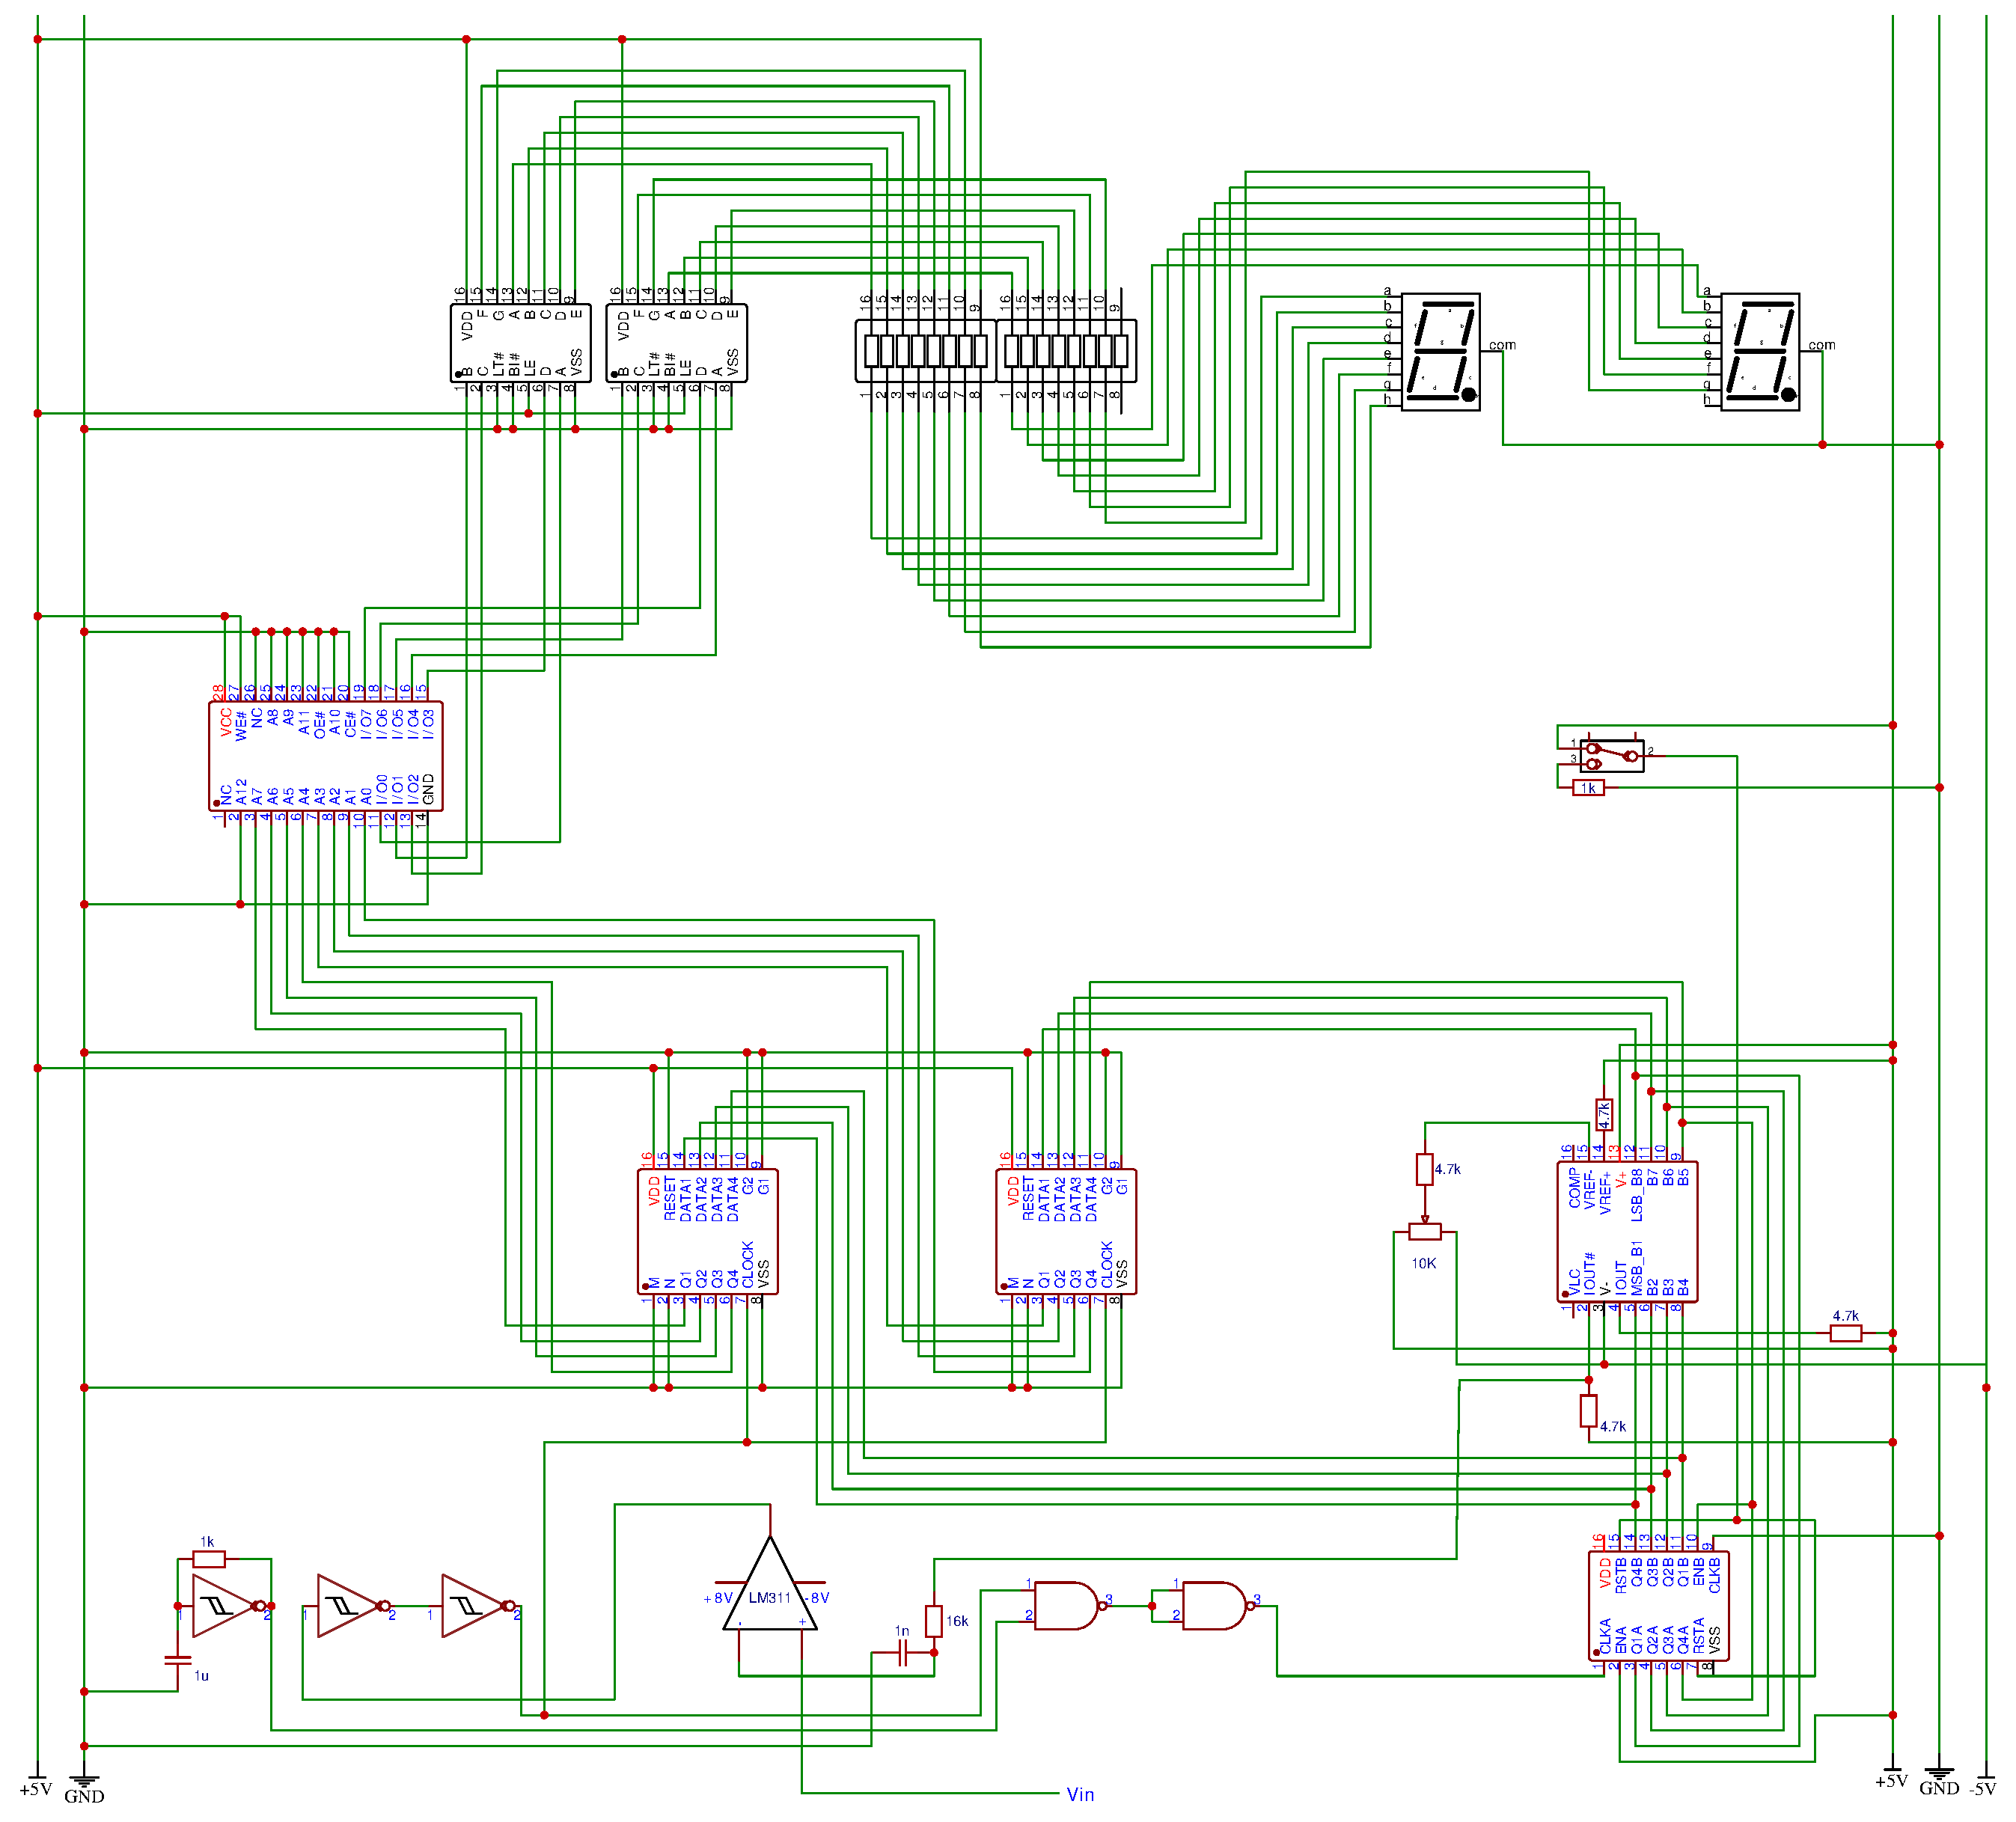
\includegraphics[width=\textwidth]{images/fullSchematic.pdf}
    \caption{Full Schematic}
    \label{fig:fullSchematic}
\end{figure}

\chapter{Final Physical Layout}
\begin{figure}[H]
    \centering
    \includegraphics[width=\textwidth, angle=270 ]{images/finalLayout.jpg}
    \caption{Final layout of the circuit}
    \label{fig:finalLayout}
\end{figure}




\chapter{Full Components list}
\section{Resistors}
\begin{itemize}
    \item 2 $220\Omega$ 8-way resistor packs
    \item 1 $380\Omega$ 
    \item 1 $1K\Omega$
    \item 4 $4.7K\Omega$
    \item 1 $10K\Omega$ rotary potentiometer
    \item 1 $10K\Omega$
    \item 1 $16K\Omega$
\end{itemize}

\section{Capacitors}
\begin{itemize}
    \item 7 $1\mu F$
    \item 1 $1nF$
\end{itemize}

\section{Integrated Circuit Chips}
\begin{itemize}
    \item 1 CD40106, Hex Schmitt Inverter, https://www.ti.com/lit/ds/symlink/cd40106b.pdf
    \item 1 LM311, Comparator, https://www.ti.com/lit/ds/symlink/lm311.pdf
    \item 1 CD4011, Quad NAND Gates, https://www.ti.com/lit/ds/symlink/cd4011b.pdf
    \item 1 CD4520, Dual Binary Up-Down Counter, https://www.ti.com/lit/ds/symlink/cd4520b.pdf
    \item 1 DAC0800LCN, 8-Bit Digital To Analogue Converter,\\ https://www.ti.com/lit/ds/symlink/dac0800.pdf
    \item 2 CD40706, 4-Bit D-Type Registers, https://www.ti.com/lit/ds/symlink/cd4076b.pdf
    \item 2 CD4511, BCD-To-7-Segment Latch Decoder Drivers,\\ https://www.ti.com/lit/ds/symlink/cd4511b.pdf
    \item 1 AT28C64B, 64K (8K x 8) Parallel EEPROM with Page Write and Software Data Protection, https://ww1.microchip.com/downloads/en/DeviceDoc/doc0270.pdf
\end{itemize}

\section{Other}
\begin{itemize}
    \item 1 Push-To-Make button
\end{itemize}




\end{document}
